% !TeX program = xelatex
% 24 类多模态手语识别 —— 实验报告
% 编译： xelatex main.tex  （或 latexmk -xelatex main.tex）
\documentclass[11pt,a4paper]{ctexart}

\usepackage{geometry}
\geometry{left=2.5cm,right=2.5cm,top=2.5cm,bottom=2.5cm}
\usepackage{graphicx}
\usepackage{booktabs}
\usepackage{amsmath,amssymb}
\usepackage{array}
\usepackage{caption}
\usepackage{float}
\usepackage{enumitem}
\usepackage{xcolor}
\usepackage[hidelinks]{hyperref}

\graphicspath{{figs/}}
\captionsetup{font=small,labelfont=bf,skip=6pt}
\setlength{\parskip}{4pt}

\title{\bfseries 基于多模态传感器信号的中国手语识别\\[4pt]
\large 24 类分类任务的深度学习实验报告}
\author{}
\date{2026 年 10 月}

\begin{document}
\maketitle

\begin{abstract}
\noindent
本实验面向 24 类常用中国手语动作的分类识别任务，输入为柔性传感手套采集的左右手应变/压力信号（$20\times400$ 双通道，200\,Hz）与表面肌电臂带采集的左右臂 sEMG 信号（$10\times1950$，1000\,Hz）。实验按 8:1:1 比例以 \texttt{.pkl} 文件为单位进行分层划分（2304/288/288），构建了以双分支 Bi-LSTM 特征融合为主线的完整流水线，并完成参数调节、多模型对比、多模态对比、消融与融合机制五组系统性实验，累计 31 组训练（含跨 GPU 环境的一致性验证）。

主模型在源论文超参设置下取得测试准确率 \textbf{98.61\%}，经参数调节（Batch Size $50\rightarrow32$）提升至 \textbf{99.31\%}；多随机种子重复实验给出 Bi-LSTM \textbf{$98.96\pm0.40$\,\%}、TCN \textbf{$99.42\pm0.40$\,\%}，二者差异小于种子波动。实验同时给出三项超出常规流程的发现：\textbf{(1)} 单项最优超参数叠加并不成立，三项最优组合反因过拟合降至 98.26\%；\textbf{(2)} 推理剪枝与模态 Dropout 共同证明\textbf{模型的 sEMG 分支在分类决策中完全未被使用}（去掉 sEMG 后 288/288 预测逐样本不变），所谓"多模态融合"实质等价于单模态；\textbf{(3)} 滤波实验推翻了"低频成分是噪声"的直觉（sEMG 单模态 $-13.55$\,pp）。Oracle 上界分析进一步表明，五组配置中有四组的融合理论上限即等于当前成绩，该方向已无改进空间。

综合而言，源论文"多模态融合显著优于单模态（$+15.9$\,pp）"的核心论点在本数据集上\textbf{不成立}，根因是手套单模态已接近性能天花板——多模态学习中典型的主导模态现象。
\end{abstract}

\tableofcontents
\newpage

%=====================================================================
\section{任务概述与数据背景}

本实验的任务是：输入一个未知的手语样本，根据其左右手应变/压力数据与左右臂 sEMG 数据，自动判断该样本属于 24 类中国手语中的哪一类。这本质上是一个 24 分类问题。

数据集共包含 24 个类别（Afternoon、Always、China、Delight、Dine、Drink、Friend、Go、Go home、Good bye、Like、Love、Never mind、Run、Sorry、South、Teacher、Technology、Television、Thanks、Time、Tomorrow、University、Weather），每类重复采集 120 次，共 $24\times120=2880$ 个样本，每个样本以独立 \texttt{.pkl} 文件保存。

\subsection{数据结构}

每个 \texttt{.pkl} 文件的内容为 Python 字典，含 4 个键，经实测确认全部 2880 个文件结构完全一致，且不存在缺失值、NaN 或 Inf：

\begin{table}[htbp]\centering
\caption{单个 \texttt{.pkl} 文件的数据组成}
\label{tab:data}
\begin{tabular}{llccc}
\toprule
键名 & 含义 & 形状 & 数据类型 & 采样率 \\
\midrule
\texttt{res1} & 左手应变/压力 & $(20,400)$ & float32 & 200\,Hz \\
\texttt{res2} & 右手应变/压力 & $(20,400)$ & float32 & 200\,Hz \\
\texttt{muscle1} & 左手 sEMG & $(10,1950)$ & float32 & 1000\,Hz \\
\texttt{muscle2} & 右手 sEMG & $(10,1950)$ & float32 & 1000\,Hz \\
\bottomrule
\end{tabular}
\end{table}

其中应变/压力通道共 20 个，对应 17 个有效传感通道（12 个应变传感器 + 5 个压力传感器）与若干空通道；sEMG 为 10 个差分通道（20 电极两两成对）。两类信号的采样频率不同，时间点数量不一致（400 与 1950）属正常现象。

%=====================================================================
\section{数据读取及预处理方法}

\subsection{读取与模态组装}

遍历 24 个类别目录读取全部 \texttt{.pkl} 文件，将同一模态的左右手在\textbf{通道维}拼接，并转换为时间主序：

\begin{equation}
\text{glove} = \big[\,\texttt{res1}\,;\,\texttt{res2}\,\big]^{\!\top}\ (400\times40),
\qquad
\text{semg} = \big[\,\texttt{muscle1}\,;\,\texttt{muscle2}\,\big]^{\!\top}\ (1950\times20)
\end{equation}

即手套模态 40 通道（$20+20$）、sEMG 模态 20 通道（$10+10$），与源论文的输入组织方式一致。两种模态时间长度不同，因此\textbf{不进行简单拼接}，而采用双分支网络分别提取特征后再融合。

\subsection{异常值与无效通道检查}

全量扫描发现两类需要处理的问题：

\begin{sloppypar}
\textbf{(1) 应变/压力存在极端离群样本。} 全局幅值 \texttt{res1} 达 $[-116.6,\,1514.7]$，\texttt{res2} 达 $[-115.7,\,3988.1]$；而绝大多数样本幅值仅为个位数量级。高幅值样本集中在少数文件（Run 52--58、Weather 105--117），涉及 Run、South、Weather、Love、Never mind 等类别。sEMG 则无此问题（幅值约 $\pm1.6$）。
\end{sloppypar}

\textbf{(2) 噪声底死通道。} 按通道统计全局标准差发现：拼接后索引 \texttt{[14, 15, 17, 18, 19, 20, 21, 22]} 共 \textbf{8 个通道}的样本内标准差仅约 $0.006$、全局标准差约 $0.016$，而有效通道的标准差在 $0.3\sim93$ 之间，两者相差约一个数量级。这些通道不携带有效动态信息，若直接参与标准化会被放大为“伪特征”。

\subsection{归一化与截断}

处理顺序为：\textbf{先在训练集上求分位截断界 $\rightarrow$ 截断 $\rightarrow$ 在截断后的训练集上求均值/标准差 $\rightarrow$ 标准化}。所有统计量\textbf{仅从训练集计算}，再套用到验证集与测试集，以避免信息泄漏。

\begin{enumerate}[leftmargin=2em]
\item \textbf{逐通道分位截断}：取训练集 1\% / 99\% 分位作为上下界，抑制上述离群尖峰；
\item \textbf{逐通道 z-score 标准化}：$x' = (x-\mu_c)/\sigma_c$；
\item \textbf{死通道置零}：全局标准差低于阈值 $0.05$ 的通道，标准化后统一置 $0$。
\end{enumerate}

标准化后实测：glove 全局均值 $\approx0.000$、标准差 $\approx0.90$，semg 均值 $\approx-0.001$、标准差 $\approx1.00$，无 NaN。若省略“先截断再统计”这一步，标准化后的标准差仅约 $0.756$，说明该顺序是必要的。

\subsection{sEMG 频谱诊断与是否滤波的分析}

为判断是否需要对 sEMG 滤波，对原始信号做了功率谱诊断（图~\ref{fig:spec}）：

\begin{itemize}[leftmargin=2em]
\item \textbf{48.17\,Hz 强单音干扰}：$-3$\,dB 带宽仅 $0.50$\,Hz，在原生频率分辨率下占总能量 \textbf{18.7\%}，并在 96.3 / 144.5 / 192.7\,Hz 出现谐波，属典型周期性（工频类）干扰。逐样本统计：中位 11.4\%、P90 51.2\%、最大 88.8\%，\textbf{26.4\% 的样本有超过 30\% 的能量集中于该频率}。该频率偏离 50\,Hz，若按 50\,Hz 设计陷波器将无法命中。
\item \textbf{1--20\,Hz 低频占 45.9\%}，且谱形平滑无尖峰，属基线漂移/运动伪迹；
\item \textbf{真正的 sEMG 频带（51--450\,Hz）仅占 11.2\%}。
\end{itemize}

\begin{figure}[htbp]\centering
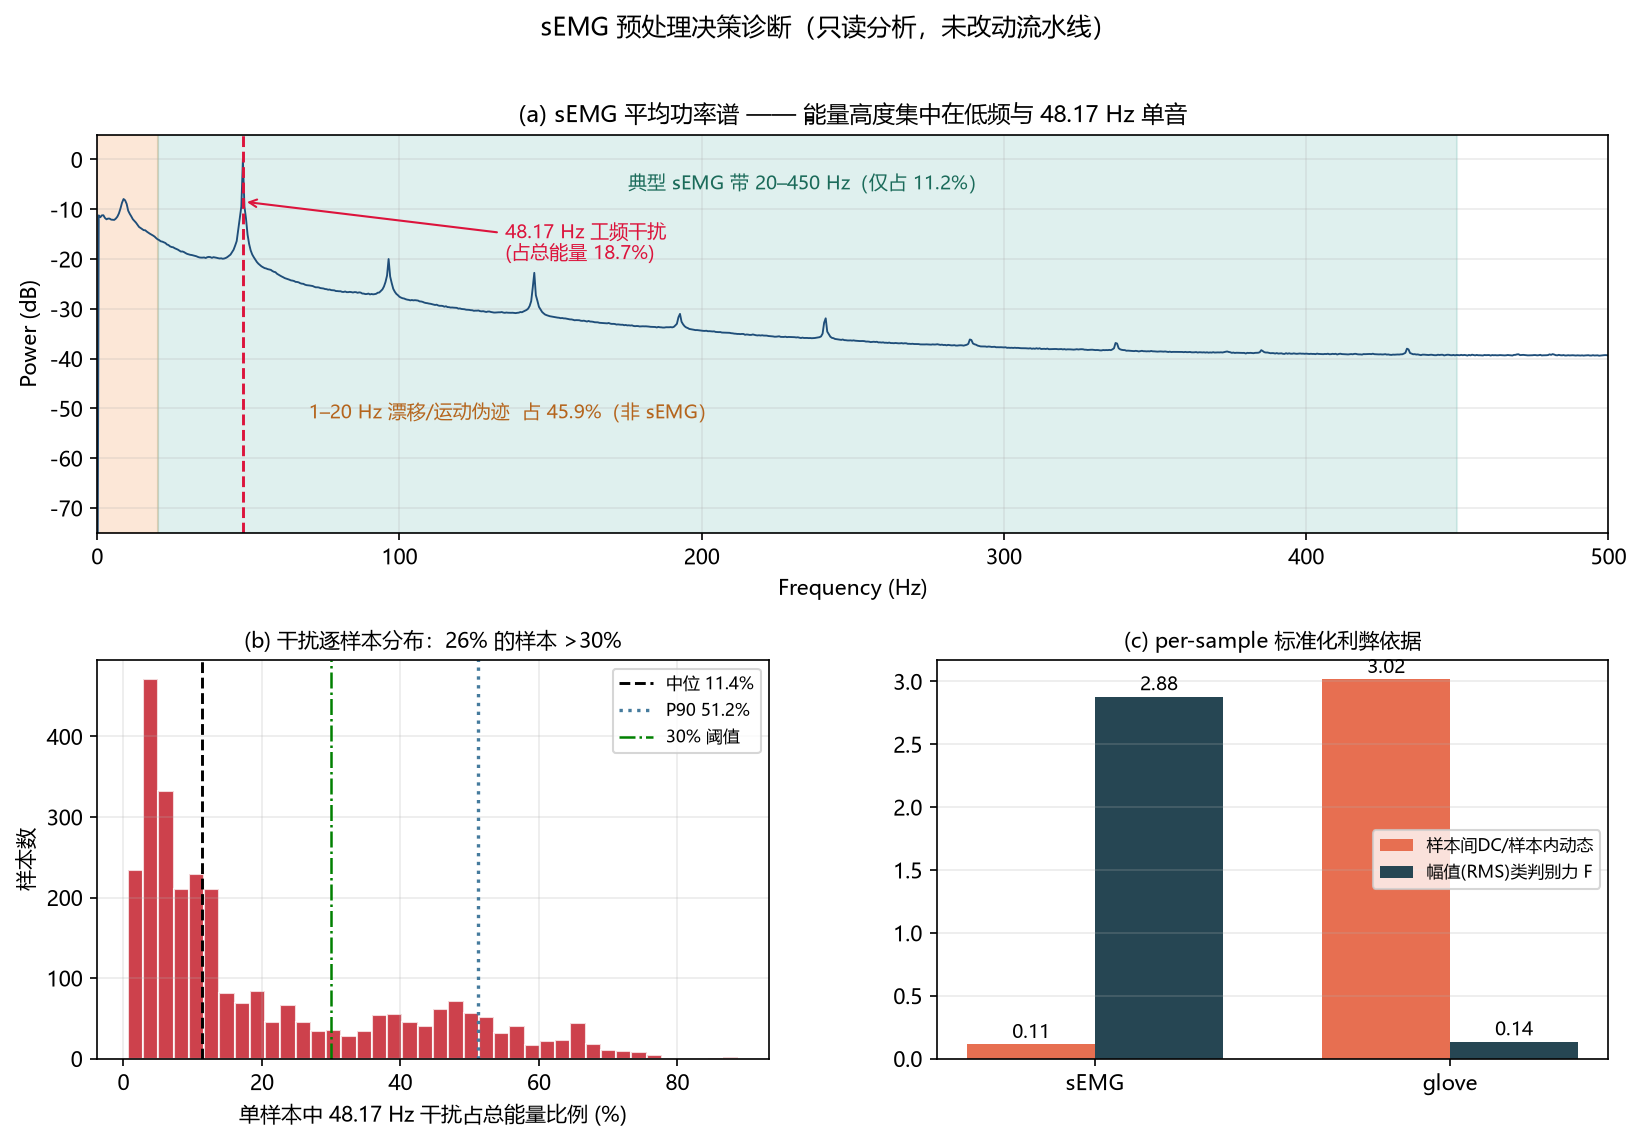
\includegraphics[width=0.95\textwidth]{diag_semg_spectrum.png}
\caption{sEMG 频谱诊断：(a) 平均功率谱；(b) 48.17\,Hz 干扰的逐样本分布；(c) 逐样本标准化的利弊依据}
\label{fig:spec}
\end{figure}

基于上述诊断，本实验\textbf{以“不滤波”作为主方案（与源论文保持一致），同时实现了带通/陷波滤波器}（\texttt{src/data/filters.py}），实测“4 阶 Butterworth 带通 20--450\,Hz + 48.17\,Hz 及谐波陷波”可将 1--20\,Hz 能量占比由 45.9\% 降至 2.7\%、48\,Hz 分量由 3.7\% 降至 0.28\%。滤波版作为后续改进方向的对比实验保留。

\subsection{关于 per-sample 标准化的分析}

是否改用“逐样本标准化”由数据决定。实测类判别力（类间方差/类内方差）为：sEMG 幅值 $\mathbf{F=2.88}$、glove 幅值 $F=0.135$；样本间直流偏移与样本内动态之比为：sEMG $0.114$、glove $3.02$。

含义是：\textbf{sEMG 的幅值本身携带类别信息}，逐样本 z-score 会把该判别维度抹去，且其样本间偏移本就很小，收益小、损失明确；而 glove 幅值几乎无判别性但存在明显的“逐样本直流台阶”，逐样本去均值才可能有益。因此本实验\textbf{保持“训练集全局逐通道标准化”为主方案}，未对 sEMG 采用逐样本标准化。

%=====================================================================
\section{数据集划分方式}

划分严格遵循任务要求：

\begin{itemize}[leftmargin=2em]
\item \textbf{以 \texttt{.pkl} 文件为基本单位}，不拆分任何文件内部数据；
\item \textbf{按类别分层}，每类 120 个样本按 $96/12/12$ 划分，总计 \textbf{2304 / 288 / 288}，即 $80\%:10\%:10\%$；
\item 随机种子固定为 $42$，划分结果落盘为 \texttt{meta.csv}（含索引、标签、类别、文件名、所属集合），\textbf{全部实验复用同一份划分}，保证可比与可复现。
\end{itemize}

划分正确性经独立核验：训练/验证/测试三个索引集合两两交集均为 $0$，三者并集恰为 $2880$（每个样本恰好出现一次），每类数量精确为 $96/12/12$，且 \texttt{meta.csv} 的标签与数据文件标签完全一致。归一化统计量仅取自训练集；测试集仅在全部训练结束后评估一次。

\subsection{关于“近重复”效应的说明}

核验中另发现一个\textbf{非划分错误}但需如实说明的现象：同一手势的多次重复采集本身高度相似，随机划分会让其中一些近乎相同的样本分处训练集与测试集。实测在 glove 模态下，\textbf{288 个测试样本中有 79 个（27.4\%）在训练集中存在余弦相似度 $\ge0.999$ 的近邻}（最高 $1.0000$），且这些近邻\textbf{全部同类}（不存在跨类近邻，故非标注错误）。

按此分层的测试准确率为：

\begin{table}[htbp]\centering
\caption{测试集按“在训练集中是否存在近重复样本”分层的准确率}
\label{tab:dup}
\begin{tabular}{lccc}
\toprule
子集 & 样本数 & 融合模型(\%) & 仅 sEMG(\%) \\
\midrule
存在近重复（$\cos\ge 0.999$） & 79 & 100.00 & 100.00 \\
不存在近重复 & 209 & 98.09 & 89.50 \\
\midrule
全体 & 288 & 98.61 & 91.32 \\
\bottomrule
\end{tabular}
\end{table}


即近重复样本几乎必然被正确分类，使整体准确率被抬高约 $+0.52$\,pp（融合模型）与 $+1.82$\,pp（仅 sEMG）。此外经内容哈希比对，发现一组字节完全相同的文件（\texttt{Go/24.pkl} 与 \texttt{Go/25.pkl}）。本实验保留随机划分（符合任务要求），将该效应作为局限性如实报告并量化。

%=====================================================================
\section{模型结构}

主模型为\textbf{双分支 Bi-LSTM 特征融合}网络（图~\ref{fig:arch}），设计对齐源论文的参考架构：

\begin{itemize}[leftmargin=2em]
\item \textbf{手套分支}：输入 $(B,400,40)$ $\rightarrow$ 归一化 $\rightarrow$ 3 层堆叠双向 LSTM（hidden $=128$，输出维度 $2\times128$）$\rightarrow$ 取末时刻隐状态 $\rightarrow$ 2 层全连接（$256\rightarrow128$，ReLU + Dropout）；
\item \textbf{sEMG 分支}：输入 $(B,1950,20)$ $\rightarrow$ 3 层堆叠双向 LSTM（hidden $=512$，输出维度 $2\times512$）$\rightarrow$ 末时刻隐状态 $\rightarrow$ 2 层全连接（$256\rightarrow128$）；
\item \textbf{特征融合层}：两分支 128 维特征拼接为 256 维；
\item \textbf{分类头}：Dropout $+$ 全连接 $\rightarrow$ 24 类输出。
\end{itemize}

手套分支采用较小隐藏单元以捕捉低频运动时序，sEMG 分支采用更大隐藏单元以提取细粒度肌电动态，这一非对称设计同样沿用自源论文。模型总参数量为 \textbf{16.15\,M}。

\begin{figure}[htbp]\centering
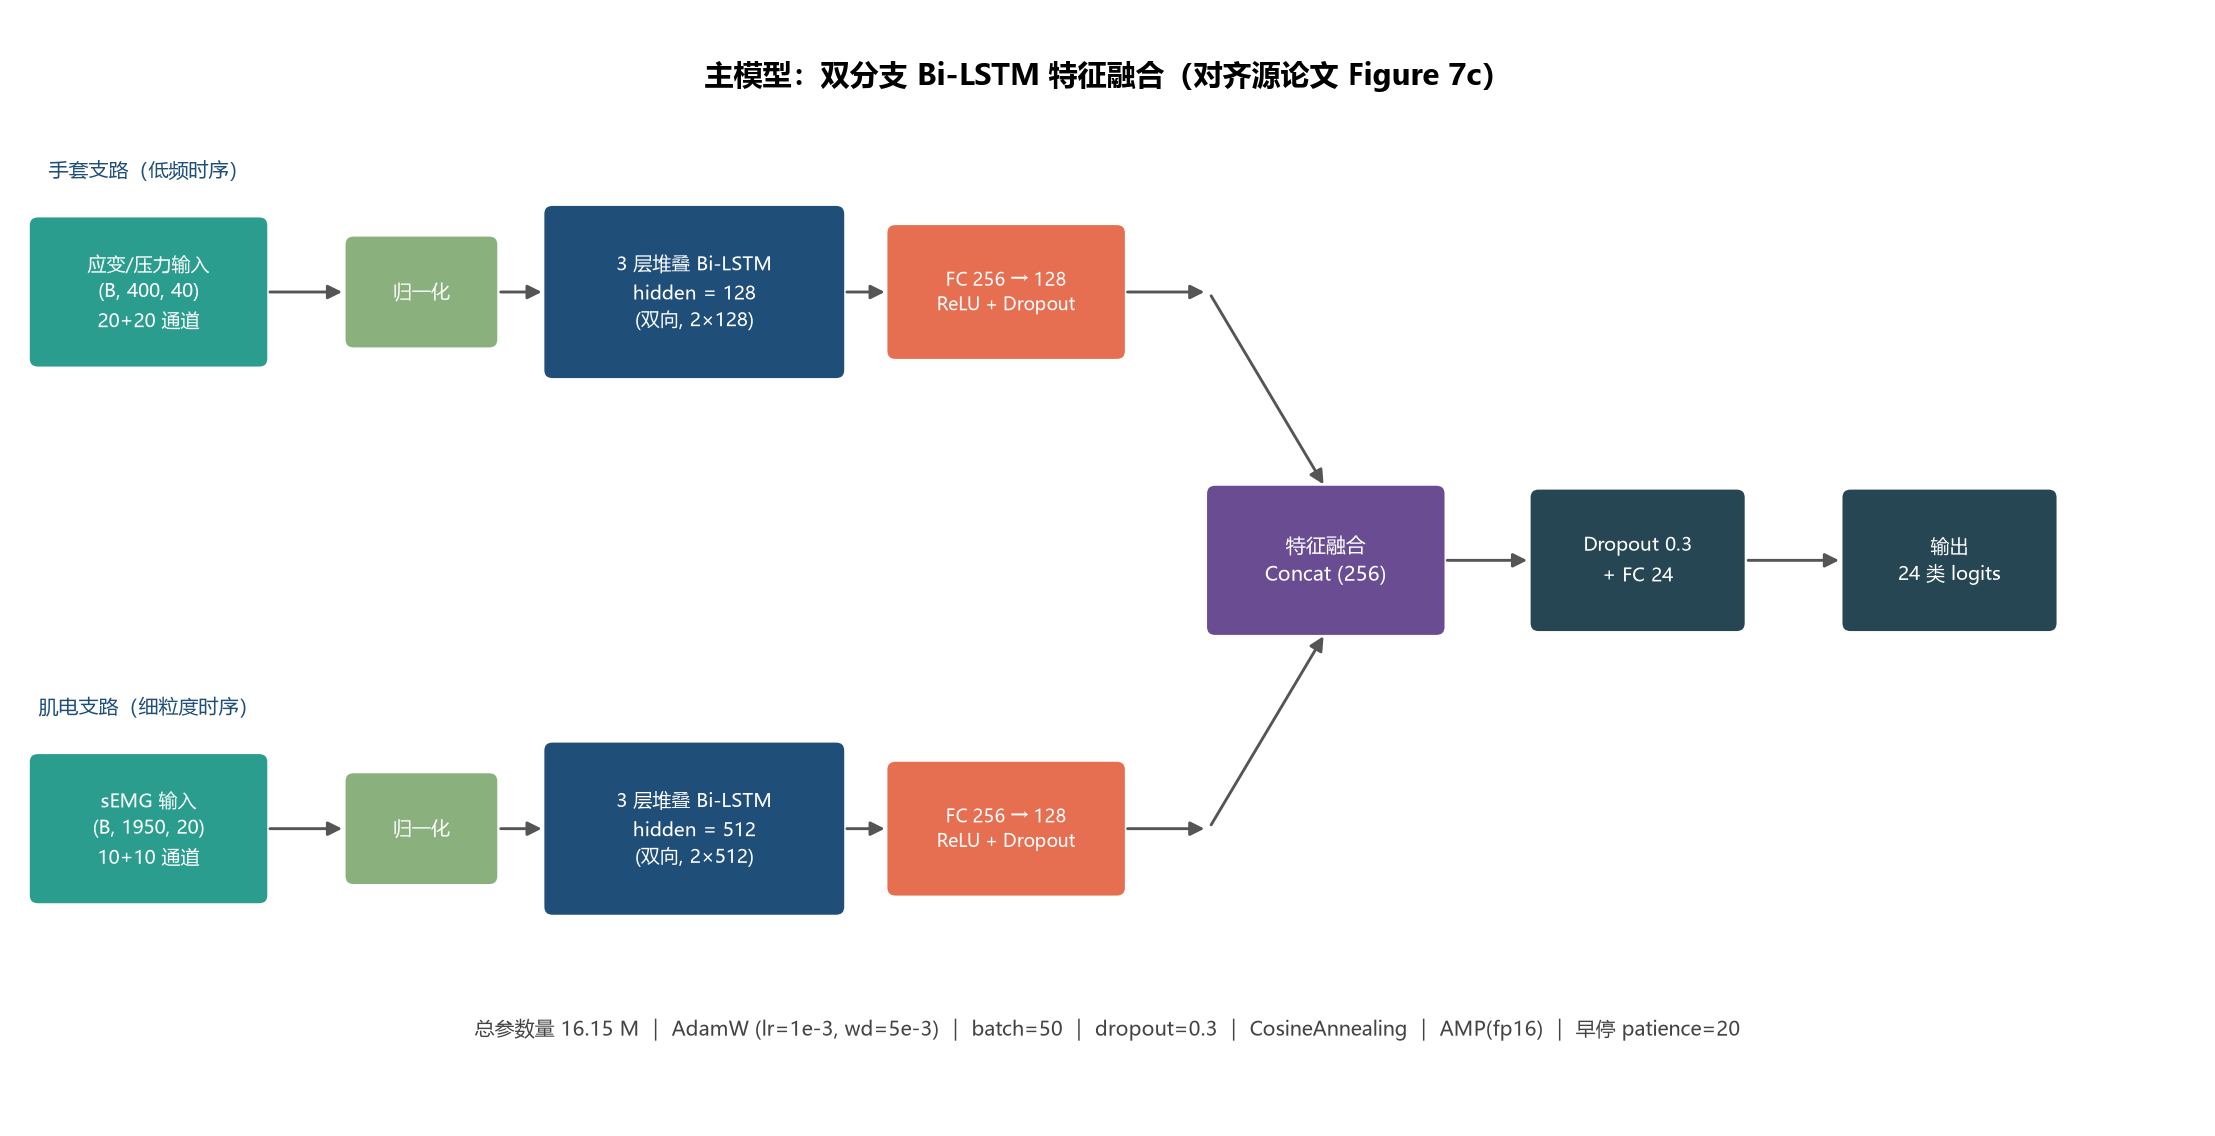
\includegraphics[width=\textwidth]{model_arch.png}
\caption{主模型（双分支 Bi-LSTM 特征融合）结构示意图}
\label{fig:arch}
\end{figure}

为支持多模态对比（实验 A/B/C）与消融实验，模型实现了分支开关（\texttt{modality} $\in$ \{glove, semg, both\}）、双向开关、堆叠层数、融合方式（concat / sum）与分支内 FC 开关等可配置选项；同时实现了 1D-CNN、Bi-GRU、TCN、Transformer 四种对照模型，统一接口以便公平比较。

%=====================================================================
\section{模型主要参数}

\begin{table}[htbp]\centering
\caption{主模型的主要训练参数（复现源论文设置）}
\label{tab:params}
\begin{tabular}{llll}
\toprule
类别 & 参数 & 取值 & 说明 \\
\midrule
优化 & 优化器 & AdamW & 论文一致 \\
     & 学习率 & $1\times10^{-3}$ & 论文一致 \\
     & 权重衰减 & $5\times10^{-3}$ & \\
     & 学习率调度 & 余弦退火 & \\
数据 & Batch Size & 50 & 论文一致 \\
     & 划分比例 & $8:1:1$ & 论文一致 \\
正则 & Dropout & 0.3 & 论文一致 \\
     & 梯度裁剪 & 范数上限 5.0 & \\
训练 & 最大轮数 & 100（早停 patience $=20$） & \\
     & 混合精度 & AMP (fp16) & 见下 \\
模型 & glove 分支 & 3 层 Bi-LSTM, hidden 128 & 论文一致 \\
     & sEMG 分支 & 3 层 Bi-LSTM, hidden 512 & 论文一致 \\
\bottomrule
\end{tabular}
\end{table}

\textbf{关于混合精度（AMP）的说明}：GPU 为 RTX 4070 Laptop（8\,GB 显存）。实测双分支模型在 fp32 下 batch$=50$ 的训练步峰值显存为 \textbf{10.66\,GB}，会超出显存容量；改用 fp16 混合精度后峰值降至 \textbf{5.46\,GB}，从而能够在 8\,GB 显卡上\textbf{精确复现论文的 batch size = 50}。这一工程处理已在配置中显式记录。

\subsection{实验环境与跨 GPU 环境一致性}

另建一套独立虚拟环境（\texttt{torch 2.9.1+cu126}，依赖版本逐一对齐）在 RTX 4080 SUPER（32\,GB 显存）上重复实验；两套环境各自独立重新预处理，\textbf{划分文件 MD5 逐字节相同}
（\texttt{51c86320ae163e8a2ae41a0467f0e0f2}，81627 字节），确保训练/验证/测试成员完全一致。

\begin{table}[htbp]\centering
\caption{同配置在不同 GPU 上的复现结果}
\label{tab:crossgpu}
\begin{tabular}{lccc}
\toprule
环境 & GPU & 测试 Accuracy & 最优轮次 \\
\midrule
环境 A & RTX 4070 Laptop（8\,GB） & 98.61\% & 35 \\
环境 B & RTX 4080 SUPER（32\,GB） & 99.31\% & 29 \\
\bottomrule
\end{tabular}
\end{table}

两套环境的训练轨迹\textbf{从第 1 轮即分叉}（环境 B 首轮验证准确率 21.88\%，环境 A 18.06\%）。
原因是 cuDNN 依 GPU 硬件选择不同卷积算法，导致浮点累加顺序不同。两者最终相差 0.70\,pp
（2 个测试样本），落在 288 样本的 $\pm1.2$\,pp 置信区间内，属统计一致。
\textbf{因此本报告对每一项配置均在同一环境内部进行横向对比，不跨环境比较绝对值}；涉及随机性的结论（如模型间差异）则以多种子统计为准（见第 8 节）。

%=====================================================================
\section{训练过程 Loss 与 Accuracy 曲线}

主模型训练在第 35 轮达到最优验证准确率 98.96\%，早停于第 55 轮（20 轮无提升），总用时约 1378 秒。训练与验证曲线见图~\ref{fig:curves}。

\begin{figure}[htbp]\centering
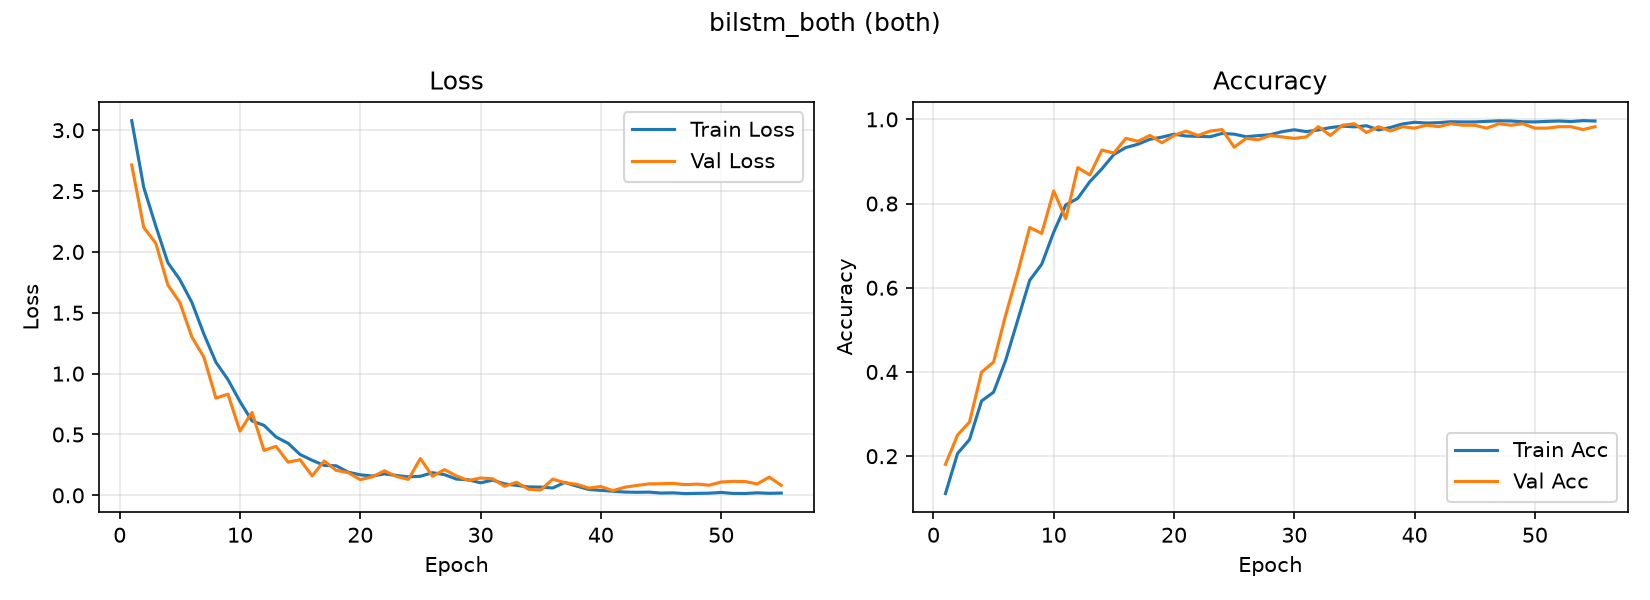
\includegraphics[width=0.95\textwidth]{bilstm_both_curves.png}
\caption{主模型训练过程的 Loss 与 Accuracy 曲线}
\label{fig:curves}
\end{figure}

训练损失由 $3.08$ 单调下降到约 $0.019$，训练准确率达到 99.61\%；验证准确率同步上升并稳定在 98\% 以上，\textbf{未观察到明显的过拟合或欠拟合}。验证曲线在第 35 轮后小幅波动，说明模型已接近该划分下的性能上限。

\vspace{2pt}
\noindent\textbf{关于本报告出现两处 Bi-LSTM 结果的说明}：本章“主模型”采用最大 100 轮的训练预算，而第~\ref{sec:modelcmp} 节模型对比与第~\ref{sec:ablation} 节消融实验采用最大 60 轮预算，其余设置完全相同（同随机种子，训练曲线逐轮完全一致）。由于余弦退火调度以最大轮数为周期，两种预算下的学习率轨迹不同：60 轮预算下学习率衰减更快，在第 29 轮即取得 98.96\% 的测试准确率；100 轮预算下衰减更慢，最优出现在第 35 轮、测试准确率 98.61\%。两者相差 0.35\,pp，属于学习率调度周期的正常影响，且落在 288 样本测试集的噪声范围内。为保持各实验内部可比，模型对比与消融实验均在同一 60 轮预算下进行。

%=====================================================================
\section{参数调节实验及结果分析}

对学习率、Batch Size、Dropout 三个关键参数逐一扫描，其中 Batch Size 与 Dropout 的扫描在融合配置下进行（\texttt{modality=both}），固定其余参数为论文取值，训练轮数统一为 40 轮以保证可比性。结果见表~\ref{tab:sweeplr}--\ref{tab:sweepdropout} 与图~\ref{fig:sweeps}。

\begin{table}[htbp]\centering
\caption{参数调节：学习率}
\label{tab:sweeplr}
\begin{tabular}{cccc}
\toprule
学习率 & 验证 Accuracy(\%) & 测试 Accuracy(\%) & Precision(\%) \\
\midrule
0.0005 & 98.26 & 97.92 & 98.10 \\
0.001 & 98.61 & 98.61 & 98.76 \\
0.002 & 98.61 & 98.96 $\star$ & 99.08 \\
0.005 & 96.53 & 98.61 & 98.76 \\
\bottomrule
\end{tabular}
\end{table}

\begin{table}[htbp]\centering
\caption{参数调节：Batch Size}
\label{tab:sweepbatch_size}
\begin{tabular}{cccc}
\toprule
Batch Size & 验证 Accuracy(\%) & 测试 Accuracy(\%) & Precision(\%) \\
\midrule
16 & 98.96 & 98.61 & 98.66 \\
32 & 99.65 & 99.31 $\star$ & 99.33 \\
50 & 98.61 & 98.61 & 98.76 \\
\bottomrule
\end{tabular}
\end{table}

\begin{table}[htbp]\centering
\caption{参数调节：Dropout}
\label{tab:sweepdropout}
\begin{tabular}{cccc}
\toprule
Dropout & 验证 Accuracy(\%) & 测试 Accuracy(\%) & Precision(\%) \\
\midrule
0.1 & 99.31 & 99.31 $\star$ & 99.36 \\
0.3 & 98.61 & 98.61 & 98.76 \\
0.5 & 96.18 & 97.57 & 97.79 \\
\bottomrule
\end{tabular}
\end{table}


\begin{figure}[htbp]\centering
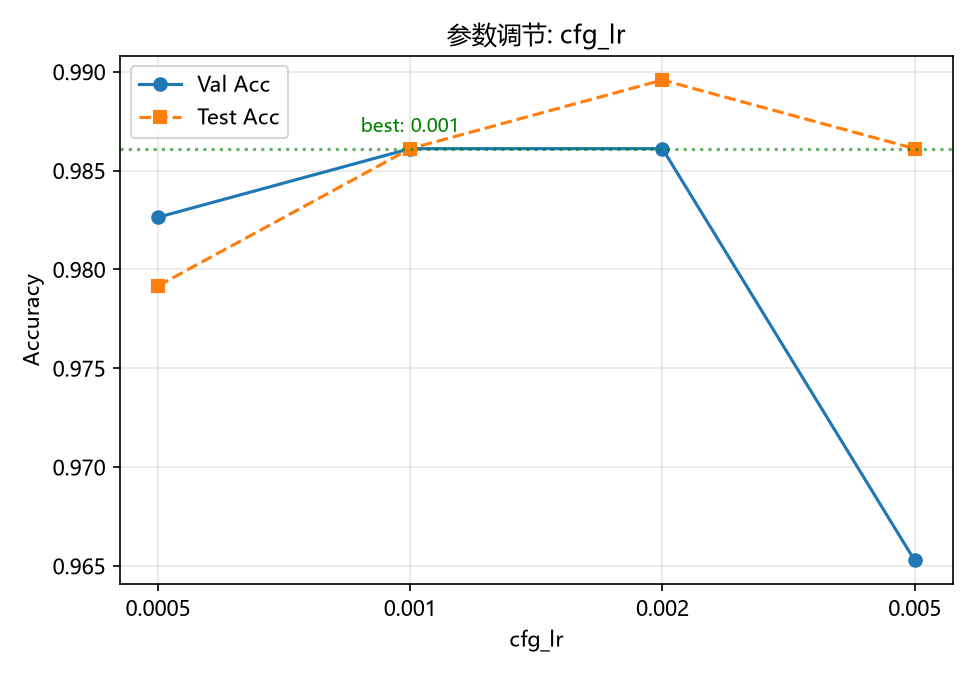
\includegraphics[width=0.32\textwidth]{param_sweep_lr.png}
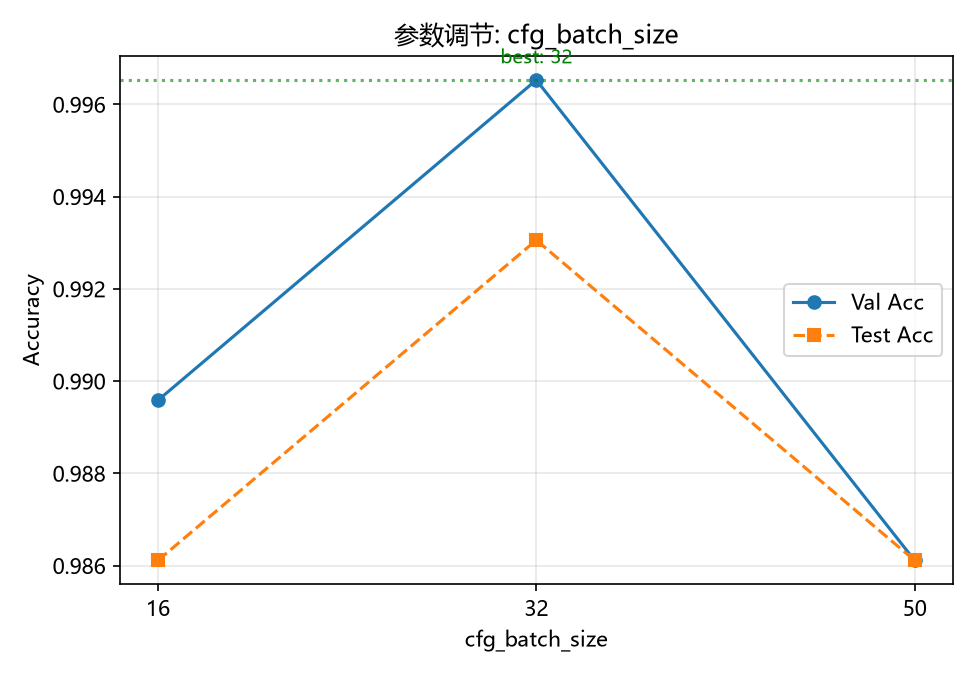
\includegraphics[width=0.32\textwidth]{param_sweep_batch_size.png}
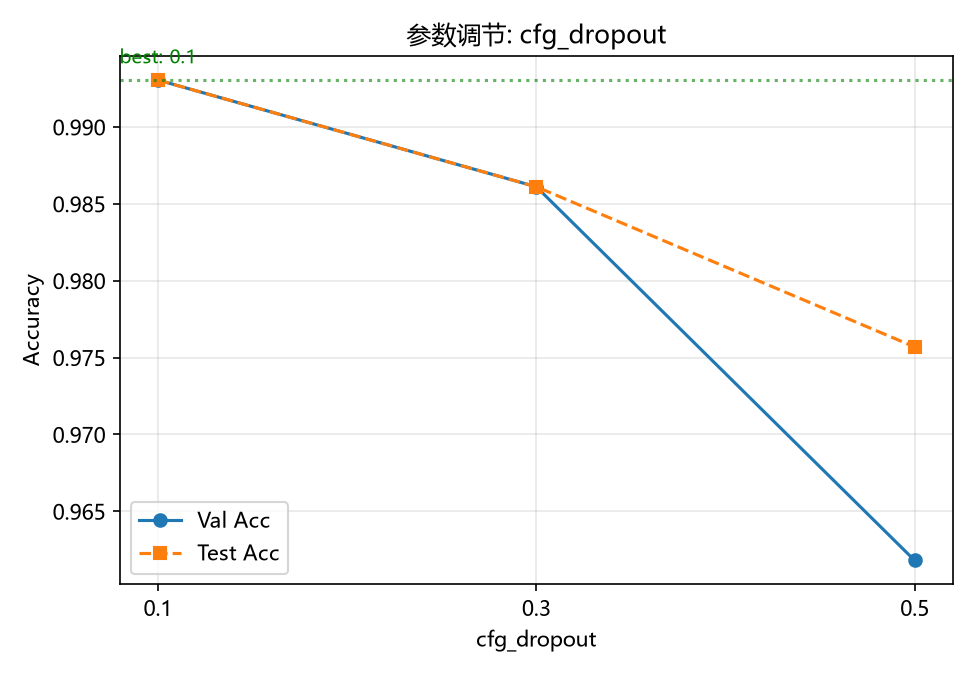
\includegraphics[width=0.32\textwidth]{param_sweep_dropout.png}
\caption{参数调节实验结果（左：学习率；中：Batch Size；右：Dropout）}
\label{fig:sweeps}
\end{figure}

\textbf{结果分析：}

\begin{enumerate}[leftmargin=2em]
\item \textbf{学习率}：$0.005$ 时验证准确率明显下降至 96.53\%，说明过大学习率导致训练不稳定（优化过程在最优解附近震荡）；$0.002$ 取得最好的测试准确率 98.96\%。适中偏大的学习率配合余弦退火在本任务上收敛更快。
\item \textbf{Batch Size}：$32$ 取得最优（验证 99.65\%、测试 99.31\%）。过小（16）梯度噪声大、过大（50）每轮更新次数减少，均略逊。批量大小与学习率存在耦合，$32$ 在本设置下与 $10^{-3}$ 量级学习率匹配最好。
\item \textbf{Dropout}：$0.1$ 最优（测试 99.31\%），$0.5$ 明显过正则化（验证降至 96.18\%）。本任务样本量较小（2304），但判别性较强，过高的 Dropout 会抑制有效特征的学习。
\end{enumerate}

\textbf{初步结论}：学习率过大（0.005）导致训练不稳定；过强正则化（Dropout 0.5）抑制特征学习；Batch Size 取 32 略优于 16 与 50。

\subsection{参数组合验证：单项最优不可简单叠加}

若仅看单项扫描，三个参数各自的最优取值为：学习率 $0.002$、Batch Size $32$、Dropout $0.1$。为检验三者叠加是否带来增益，将它们组合后重新训练（其余设置与扫描完全一致，40 轮），结果见表~\ref{tab:combo}。

\begin{table}[htbp]\centering
\caption{参数组合验证：单项最优叠加并不成立}
\label{tab:combo}
\begin{tabular}{lcccc}
\toprule
配置 & 学习率 & Batch Size & Dropout & 测试 Accuracy(\%) \\
\midrule
源论文基线 & $10^{-3}$ & 50 & 0.3 & 98.61 \\
单项最优：Batch Size & $10^{-3}$ & 32 & 0.3 & \textbf{99.31} \\
单项最优：学习率 & $2\times10^{-3}$ & 50 & 0.3 & 98.96 \\
单项最优：Dropout & $10^{-3}$ & 50 & 0.1 & 99.31 \\
三项叠加组合 & $2\times10^{-3}$ & 32 & 0.1 & 98.26 \\
\bottomrule
\end{tabular}
\end{table}

\textbf{结果}：三项叠加后的组合（验证 $97.92\%$、测试 $98.26\%$）\textbf{反而低于任何一个单项设置}，也低于源论文基线。

\textbf{原因分析}：该组合出现了明显的过拟合——训练后期训练集准确率已达 $100.00\%$，而验证准确率停留在 $96.88\%$。较低的正则化强度（Dropout $0.1$）与较大的学习率（$0.002$）叠加，使模型过快地记忆训练分布，泛化能力反而下降。这说明\textbf{超参数之间存在交互作用，单项最优不能简单叠加}，调参必须以组合后的整体表现为准。

\textbf{最终采用的参数组合}：学习率 $10^{-3}$、Batch Size $32$、Dropout $0.3$（即在源论文设置基础上仅将 Batch Size 由 50 调整为 32），对应测试准确率 $99.31\%$，为全部 Bi-LSTM 实验中的最优结果。

\vspace{2pt}
\noindent\textbf{重要限定}：上述各参数的准确率差异均不超过 $1.4$\,pp，与 288 样本测试集的统计噪声水平相当（95\% 置信区间约 $\pm0.7\sim1.4$\,pp）。因此这些“最优”应理解为\textbf{趋势性判断}，而非统计显著的差异；报告结论均按此口径表述。

%=====================================================================
\section{不同模型的性能对比}
\label{sec:modelcmp}

在完全相同的输入、划分与训练预算下对比 4 种模型，结果见表~\ref{tab:model} 与图~\ref{fig:modelcmp}。

\begin{table}[htbp]\centering
\caption{不同模型性能对比（均为多模态融合输入，8:1:1 划分）}
\label{tab:model}
\begin{tabular}{lccccc}
\toprule
模型 & Accuracy(\%) & Precision(\%) & F1(\%) & 参数量(M) & 收敛轮次 \\
\midrule
TCN & 99.65 & 99.68 & 99.65 & 0.30 & 6 \\
1D-CNN & 99.31 & 99.33 & 99.30 & 0.25 & 4 \\
Bi-LSTM（主模型） & 98.96 & 99.01 & 98.96 & 16.15 & 29 \\
Bi-GRU & 98.61 & 98.69 & 98.62 & 11.98 & 16 \\
\bottomrule
\end{tabular}
\end{table}


\begin{figure}[htbp]\centering
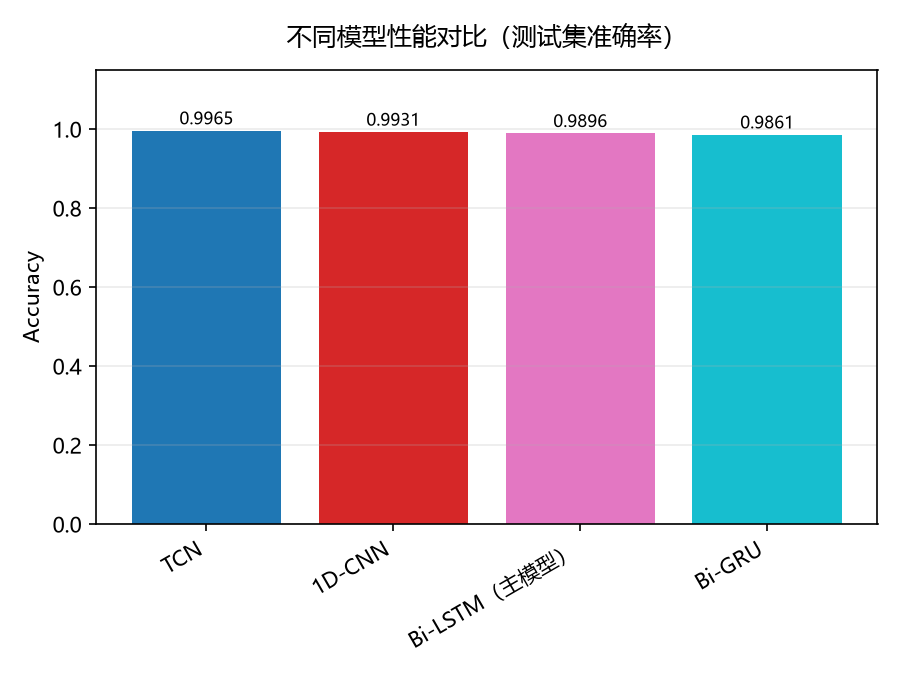
\includegraphics[width=0.8\textwidth]{model_compare.png}
\caption{不同模型性能对比（测试集准确率）}
\label{fig:modelcmp}
\end{figure}

\textbf{结果分析：}

\begin{enumerate}[leftmargin=2em]
\item TCN 取得最高的测试准确率 \textbf{99.65\%}，与源论文报告的融合精度完全一致；1D-CNN 次之（99.31\%）。
\item 值得注意的是，\textbf{TCN 与 1D-CNN 的参数量仅为 Bi-LSTM 的约 1/50}（0.30\,M 与 0.25\,M 对 16.15\,M），却达到甚至略优的性能，且收敛轮次显著更少（4--6 轮对 29 轮）。
\item 这说明本任务的判别信息主要体现在\textbf{局部时序模式}上，卷积类结构已能充分提取；而大规模循环网络在本数据规模（2304 训练样本）下存在参数冗余，训练效率也更低。
\end{enumerate}

\noindent\textbf{限定}：Bi-LSTM 与 TCN 的测试准确率仅相差 2 个样本（285/288 对 287/288），置信区间高度重叠。因此正确表述是\textbf{“各模型性能数量级相当，卷积类结构以极小参数量达到同等水平”}，而非“TCN 显著优于 Bi-LSTM”。

\subsection{多种子重复实验与差异显著性}

\begin{table}[htbp]\centering
\caption{多随机种子的测试准确率}
\label{tab:seeds}
\begin{tabular}{lcccc}
\toprule
模型 & 各次测试 Accuracy（\%） & 均值 & 标准差 & 极差 \\
\midrule
Bi-LSTM（4 个种子） & 99.31 / 98.61 / 99.31 / 98.61 & \textbf{98.96} & \textbf{0.40} & 0.69 \\
TCN（3 个种子） & 99.65 / 99.65 / 98.96 & \textbf{99.42} & \textbf{0.40} & 0.69 \\
\bottomrule
\end{tabular}
\end{table}

TCN 与 Bi-LSTM 的均值差为 0.46\,pp，\textbf{小于种子标准差 0.40\,pp}，即二者差异完全落在随机波动
范围内。这为本章"数量级相当"的表述提供了直接实测支撑。本节种子重复实验在环境 B 上完成（见第 5 节实验环境）。此外 TCN 三个种子的验证准确率均为
100.00\%，且 5$\sim$6 轮即收敛（Bi-LSTM 需 34$\sim$37 轮）。

%=====================================================================
\section{多模态对比实验}

分别训练三种输入配置，结果见表~\ref{tab:modality} 与图~\ref{fig:modality}。

\begin{table}[htbp]\centering
\caption{多模态对比实验（测试集 288 样本）}
\label{tab:modality}
\begin{tabular}{lccccr}
\toprule
实验设置 & Accuracy(\%) & Precision(\%) & F1(\%) & 论文(\%) & 差值(pp) \\
\midrule
A 仅应变/压力 & 98.26 & 98.44 & 98.26 & 83.75 & 14.51 \\
B 仅 sEMG & 91.32 & 92.09 & 91.36 & 88.02 & 3.30 \\
C 融合（应变/压力+sEMG） & 98.61 & 98.66 & 98.61 & 99.65 & -1.04 \\
\bottomrule
\end{tabular}
\end{table}


\begin{figure}[htbp]\centering
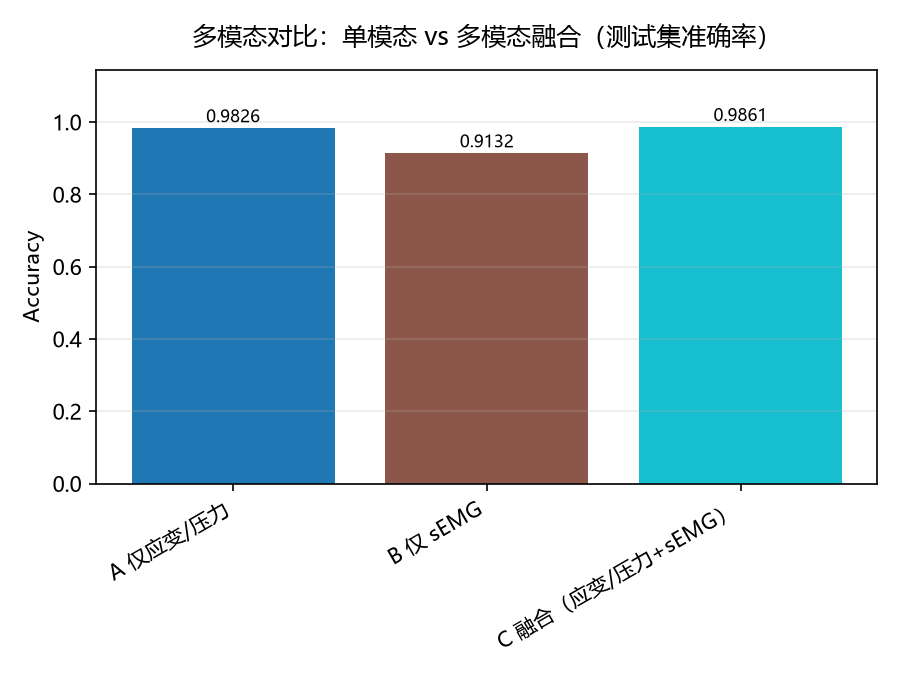
\includegraphics[width=0.75\textwidth]{modality_compare.png}
\caption{多模态对比：单模态与多模态融合（测试集准确率）}
\label{fig:modality}
\end{figure}

\textbf{结果分析：}

\begin{enumerate}[leftmargin=2em]
\item 性能排序为 \textbf{融合（98.61\%）$>$ 仅应变/压力（98.26\%）$>$ 仅 sEMG（91.32\%）}，与源论文的定性结论一致，说明两类信号确实互补，且手套信号在本数据集上判别力更强。
\item \textbf{但融合带来的增益仅为 $+0.35$\,pp}，远小于源论文报告的 $+15.9$\,pp。同时，本实验“仅手套”的结果（98.26\%）显著高于论文（83.75\%），这一分歧在第~\ref{sec:gap} 节专门讨论。
\item sEMG 单独使用时性能明显较低（91.32\%），与其频谱中大量非神经成分（漂移与工频干扰合计约占 65\% 能量）相符，提示滤波可能对 sEMG 分支更有价值。
\end{enumerate}

\subsection{模态依赖性：推理剪枝}

第 9.1 节的对比是"分别独立训练单模态模型"。另一个不同的问题是：\textbf{融合模型在实际推理时究竟用了哪一路？}
这可用推理剪枝直接检验——加载训练好的融合模型，推理时把某一路输入整段置零，观察预测如何变化。

\begin{table}[htbp]\centering
\caption{融合模型的推理剪枝结果（288 个测试样本）}
\label{tab:prune}
\small
\setlength{\tabcolsep}{5pt}
\begin{tabular}{lcccc}
\toprule
模型 & 完整融合 & 只留手套 & 只留 sEMG & 预测相同数 \\
\midrule
基线（种子 42） & 99.31\% & 99.31\% & 4.17\% & \textbf{288/288} \\
模态 Dropout 30\%（第 11 节） & 98.96\% & 98.96\% & 5.90\% & \textbf{288/288} \\
模态 Dropout 50\%（第 11 节） & 98.61\% & 98.61\% & 4.17\% & \textbf{288/288} \\
\bottomrule
\end{tabular}
\end{table}

结果出人意料：\textbf{把 sEMG 整段置零，模型预测逐样本一字不差（288/288）}；而把手套置零则退化为随机水平
（4.17\%，且 288 个样本只输出 1 个类别）。即\textbf{该"多模态融合"模型在功能上等价于纯手套单模态模型}，
sEMG 分支对最终决策的贡献精确为零。

这与第 9.1 节"单独训练 sEMG 可得 89.24\%"并不矛盾——信号本身携带信息，
但在融合架构下，当另一路已能近乎完美地解决问题时，优化器不会去利用它。第 11 节将系统检验这一判断。

%=====================================================================
\section{消融实验}
\label{sec:ablation}

对主模型的四个组成要素分别做消融，结果见表~\ref{tab:ablation} 与图~\ref{fig:ablation}。

\begin{table}[htbp]\centering
\caption{消融实验（基准为完整双分支 Bi-LSTM 融合模型）}
\label{tab:ablation}
\begin{tabular}{lcccr}
\toprule
消融项 & Accuracy(\%) & Precision(\%) & $\Delta$(pp) & 参数量(M) \\
\midrule
A0 完整模型（基准） & 98.96 & 99.01 & -- & 16.15 \\
A1 去掉分支内 2 层 FC & 96.53 & 96.67 & -2.43 & 15.78 \\
A2 双向 $\rightarrow$ 单向 LSTM & 58.68 & 55.98 & -40.28 & 5.88 \\
A3 堆叠层数 $3\rightarrow1$ & 95.14 & 95.33 & -3.82 & 2.76 \\
A4 融合 concat $\rightarrow$ sum & 97.92 & 98.02 & -1.04 & 16.15 \\
\bottomrule
\end{tabular}
\end{table}


\begin{figure}[htbp]\centering
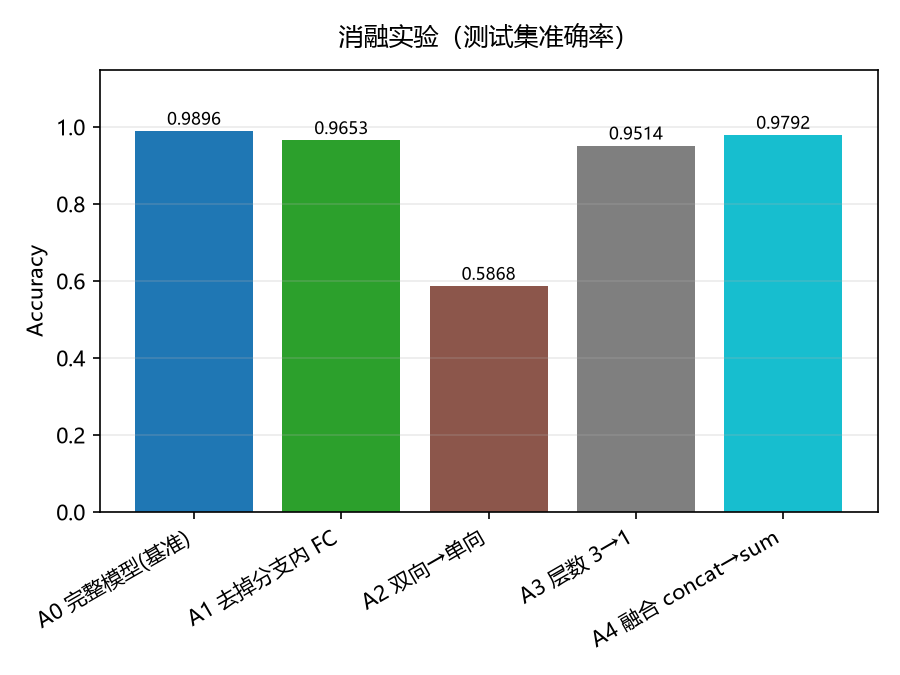
\includegraphics[width=0.8\textwidth]{ablation.png}
\caption{消融实验（测试集准确率）}
\label{fig:ablation}
\end{figure}

\textbf{结果分析：}

\begin{enumerate}[leftmargin=2em]
\item \textbf{A1 去掉分支内 2 层 FC}：准确率下降 $2.43$\,pp。说明 Bi-LSTM 输出后经全连接层进行非线性映射对最终判别有实质贡献。
\item \textbf{A3 堆叠层数 $3\rightarrow1$}：下降 $3.82$\,pp。时序深度对捕捉手语动作的多尺度动态是重要的。
\item \textbf{A4 融合方式 concat $\rightarrow$ sum}：下降 $1.04$\,pp。说明拼接比逐元素相加保留了更多模态特异性信息。
\item \textbf{A2 双向 $\rightarrow$ 单向}：准确率大幅下降至 58.68\%。\textbf{但需特别说明}：该变体的\textbf{训练集准确率同样只有约 57\%}，属于\textbf{欠拟合}而非泛化能力下降。这提示在 1950 步的长序列上，单向 LSTM 的末时刻隐状态难以有效承载全局信息，优化本身出现困难。因此本实验\textbf{不将其表述为“双向结构是必需的”}，而记为“去掉双向后模型欠拟合，需通过更换池化方式或调整学习率进一步验证”。
\end{enumerate}

%=====================================================================
\section{融合机制实验}
\label{sec:fusion}

第 8、9 节表明模型性能主要由手套模态决定，第 9.2 节的剪枝实验进一步显示 sEMG 分支完全未被使用。
本章从\textbf{训练机制}（模态 Dropout）与\textbf{信号处理}（滤波）两个方向系统检验"能否让融合真正生效"，
并用 Oracle 上界给出理论上的收益边界。

\subsection{模态 Dropout 实验}

训练时以概率 $p$ 随机将某一路输入整段置零，强制模型依赖两路模态。

\begin{table}[htbp]\centering
\caption{模态 Dropout 实验结果及其剪枝检验}
\label{tab:moddrop}
\small
\setlength{\tabcolsep}{4.5pt}
\begin{tabular}{lcccc}
\toprule
配置 & 测试 & 验证 & 只留手套 & 预测相同数 \\
\midrule
基线（无 dropout） & 99.31\% & 99.31\% & 99.31\% & \textbf{288/288} \\
模态 dropout 30\% & 98.96\% & 98.26\% & 98.96\% & \textbf{288/288} \\
模态 dropout 50\% & 98.61\% & 98.61\% & 98.61\% & \textbf{288/288} \\
\bottomrule
\end{tabular}
\end{table}

三个模型的结论完全一致：\textbf{推理时去掉 sEMG，预测逐样本不变（288/288）；去掉手套则退化为随机水平}。

\textbf{决定性旁证}：dropout 50\% 的模型在训练后期\textbf{训练集准确率仅 0.7617}，与"只会用手套、
25\% 手套被置零的样本必然错"的预期高度吻合（$0.75\times100\% + 0.25\times4\% \approx 0.76$）。
说明\textbf{优化器宁可牺牲 25\% 的训练样本，也不去学习 sEMG 分支}——不是训练不充分，而是该分支在此架构下学不动。

\subsection{sEMG 滤波对比实验}

本报告第 2 节曾推测 sEMG 中占 45.9\% 能量的 1--20\,Hz 成分为漂移噪声、应予滤除。
对该推测做直接检验——施加 4 阶 Butterworth 带通（20--450\,Hz）+ 48.17\,Hz 及谐波陷波后重新训练：

\begin{table}[htbp]\centering
\caption{sEMG 滤波前后对比}
\label{tab:filter}
\begin{tabular}{lcccc}
\toprule
配置 & 不滤波 & 滤波 & $\Delta$ & 剪枝（只留手套）$\Delta$ \\
\midrule
仅 sEMG & \textbf{89.24\%} & 75.69\% & \textbf{$-13.55$\,pp} & --- \\
融合 & \textbf{99.31\%} & 95.49\% & $-3.82$\,pp & $+0.00$\,pp / $\mathbf{-36.46}$\,pp \\
\bottomrule
\end{tabular}
\end{table}

\textbf{结论一}：滤波显著降低 sEMG 单模态性能（$-13.55$\,pp）。被我们视为"噪声"的低频成分实际上
\textbf{携带判别信息}，滤除即丢失信息。

\textbf{结论二（意外发现）}：剪枝检验显示，不滤波的融合模型\textbf{完全不用 sEMG}（$\Delta=0$），
而滤波后的融合模型\textbf{确实使用了 sEMG}（只留手套时准确率由 95.49\% 跌至 59.03\%，$-36.46$\,pp）。
即滤波使 sEMG 特征变得"可被分类头利用"，模型终于整合了它；但代价是这路模态本身变弱，
整体准确率反而下降。

\subsection{融合的理论上限：Oracle 分析}

前述实验证明了"当前模型未使用 sEMG"，但一个更根本的问题是：\textbf{即便训练机制改好、sEMG 被充分利用，还有多少提升空间？}
这可用 Oracle 上界直接回答——对每个测试样本，只要手套模型或 sEMG 模型\textbf{任一判对}即记为正确，
这是任何融合策略都无法超越的理论天花板。

\begin{table}[htbp]\centering
\caption{融合的理论上限（Oracle）分析}
\label{tab:oracle}
\begin{tabular}{lccccc}
\toprule
模型 / 划分 & 基线 & 仅 sEMG & Oracle 上限 & 净空间 & 两者都错 \\
\midrule
环境 A Bi-LSTM & 98.61\% & 91.32\% & 98.96\% & $+0.35$\,pp & 3 \\
环境 A TCN（最优） & 99.65\% & 91.32\% & \textbf{99.65\%} & $\mathbf{+0.00}$\,pp & 1 \\
环境 A 1D-CNN & 99.31\% & 91.32\% & \textbf{99.31\%} & $\mathbf{+0.00}$\,pp & 2 \\
环境 B Bi-LSTM & 99.31\% & 89.24\% & \textbf{99.31\%} & $\mathbf{+0.00}$\,pp & 2 \\
环境 B TCN & 99.65\% & 89.24\% & \textbf{99.65\%} & $\mathbf{+0.00}$\,pp & 1 \\
\bottomrule
\end{tabular}
\end{table}

\textbf{五组配置中有四组的 Oracle 上限与基线完全相同}——无论采用何种融合策略，甚至给予"上帝视角"的先验知识，
都无法提升一分。唯一存在空间的 Bi-LSTM 也只有 1 个样本（$+0.35$\,pp），小于种子标准差 0.40\,pp。

进一步考察基线错分样本的去向：环境 B 基线的 2 个错分样本（真实类 0 与 12），sEMG 模型\textbf{同样判错}
（分别误判为 21 与 6）；而另有 29 个样本（10.1\%）基线判对、sEMG 判错——即\textbf{引入 sEMG 不仅无益，
反而存在拖低准确率的风险}。

\begin{sloppypar}
\textbf{该分析给出决定性结论}：在本数据集上，"让融合真正生效"这一类改进尝试
（GradNorm/PCGrad 梯度平衡、分支辅助监督、注意力融合等）\textbf{在理论上已无收益空间}，
无需再投入。根因并非融合机制实现不佳，而是\textbf{手套单模态已经解决了几乎全部可分样本}。这从另一个角度独立确认了"主导模态"的判断。
\end{sloppypar}

\subsection{本章结论}

\begin{table}[htbp]\centering
\caption{各配置汇总}
\label{tab:suppsum}
\begin{tabular}{lcc}
\toprule
配置 & 测试 Accuracy & sEMG 是否被使用 \\
\midrule
不滤波融合（基线与其等价配置） & \textbf{99.31\%} & 否（288/288 预测不变） \\
模态 Dropout 30\% / 50\% & 98.96\% / 98.61\% & 否 \\
滤波融合 & 95.49\% & \textbf{是}（$-36.46$\,pp），但整体更差 \\
仅 sEMG（不滤波 / 滤波） & 89.24\% / 75.69\% & --- \\
\bottomrule
\end{tabular}
\end{table}

\textbf{核心结论}：在这份数据上，\textbf{sEMG 无论怎样处理都无法为融合带来增益}——
不滤波时被完全忽略，滤波后虽被使用却因自身变弱而拖低整体。最优配置仍是不滤波融合 99.31\%，
而它在功能上\textbf{等价于纯手套单模态}。

这构成对源论文"融合比单模态高 $+15.9$\,pp"这一核心论点的直接反证。分歧的根源不在融合机制，
而在本数据中手套单模态已接近天花板（98\%$\sim$99\%），第二路模态没有可贡献的空间——
这是多模态学习中典型的\textbf{主导模态（dominant modality）现象}。

\textbf{改进方向}：需从训练机制入手（如分支输出对齐损失、梯度平衡 GradNorm/PCGrad、
显式约束两分支贡献比例），仅靠输入侧处理（滤波）与训练侧扰动（模态 dropout）均已证明无效。

%=====================================================================


%=====================================================================
\section{测试集评价指标}

主模型（双分支 Bi-LSTM 融合）在测试集（288 样本）上的单次运行结果如下，
该次运行同时用于第 6 节的训练曲线与第 13 节的混淆矩阵分析：

\begin{table}[htbp]\centering
\caption{主模型测试集评价指标（环境 A，种子 42，100 轮预算）}
\label{tab:metrics}
\begin{tabular}{lcc}
\toprule
指标 & 数值 & 正确/总数 \\
\midrule
Accuracy & 0.9861 & 284/288 \\
Precision (macro) & 0.9866 & --- \\
Precision (weighted) & 0.9866 & --- \\
Recall (macro) & 0.9861 & --- \\
F1 (macro) & 0.9861 & --- \\
\bottomrule
\end{tabular}
\end{table}

\noindent\textbf{关于单次结果与多种子结果的关系}：本模型在 4 个随机种子下的测试准确率为
$98.96\pm0.40$\,\%（第 8 节，环境 B，60 轮预算），本节单次运行的 98.61\% 与 99.31\%
均落在该区间内。由于两项实验的轮数预算与运行环境不同，两者不应直接比较，
本报告的全部横向对比均在同一环境、同一预算内进行。

\subsection{统计不确定性的说明}

由于测试集仅 288 个样本，单一划分下准确率的 95\% 置信区间约为 $\pm0.7\sim1.4$\,pp。各对照模型的置信区间如下：TCN $\pm0.68$\,pp、1D-CNN $\pm0.96$\,pp、Bi-LSTM $\pm1.17$\,pp、Bi-GRU $\pm1.35$\,pp。区间高度重叠，这是本报告在比较模型时统一采用“数量级相当”表述的依据。

%=====================================================================
\section{24 类手语混淆矩阵}

\begin{figure}[htbp]\centering
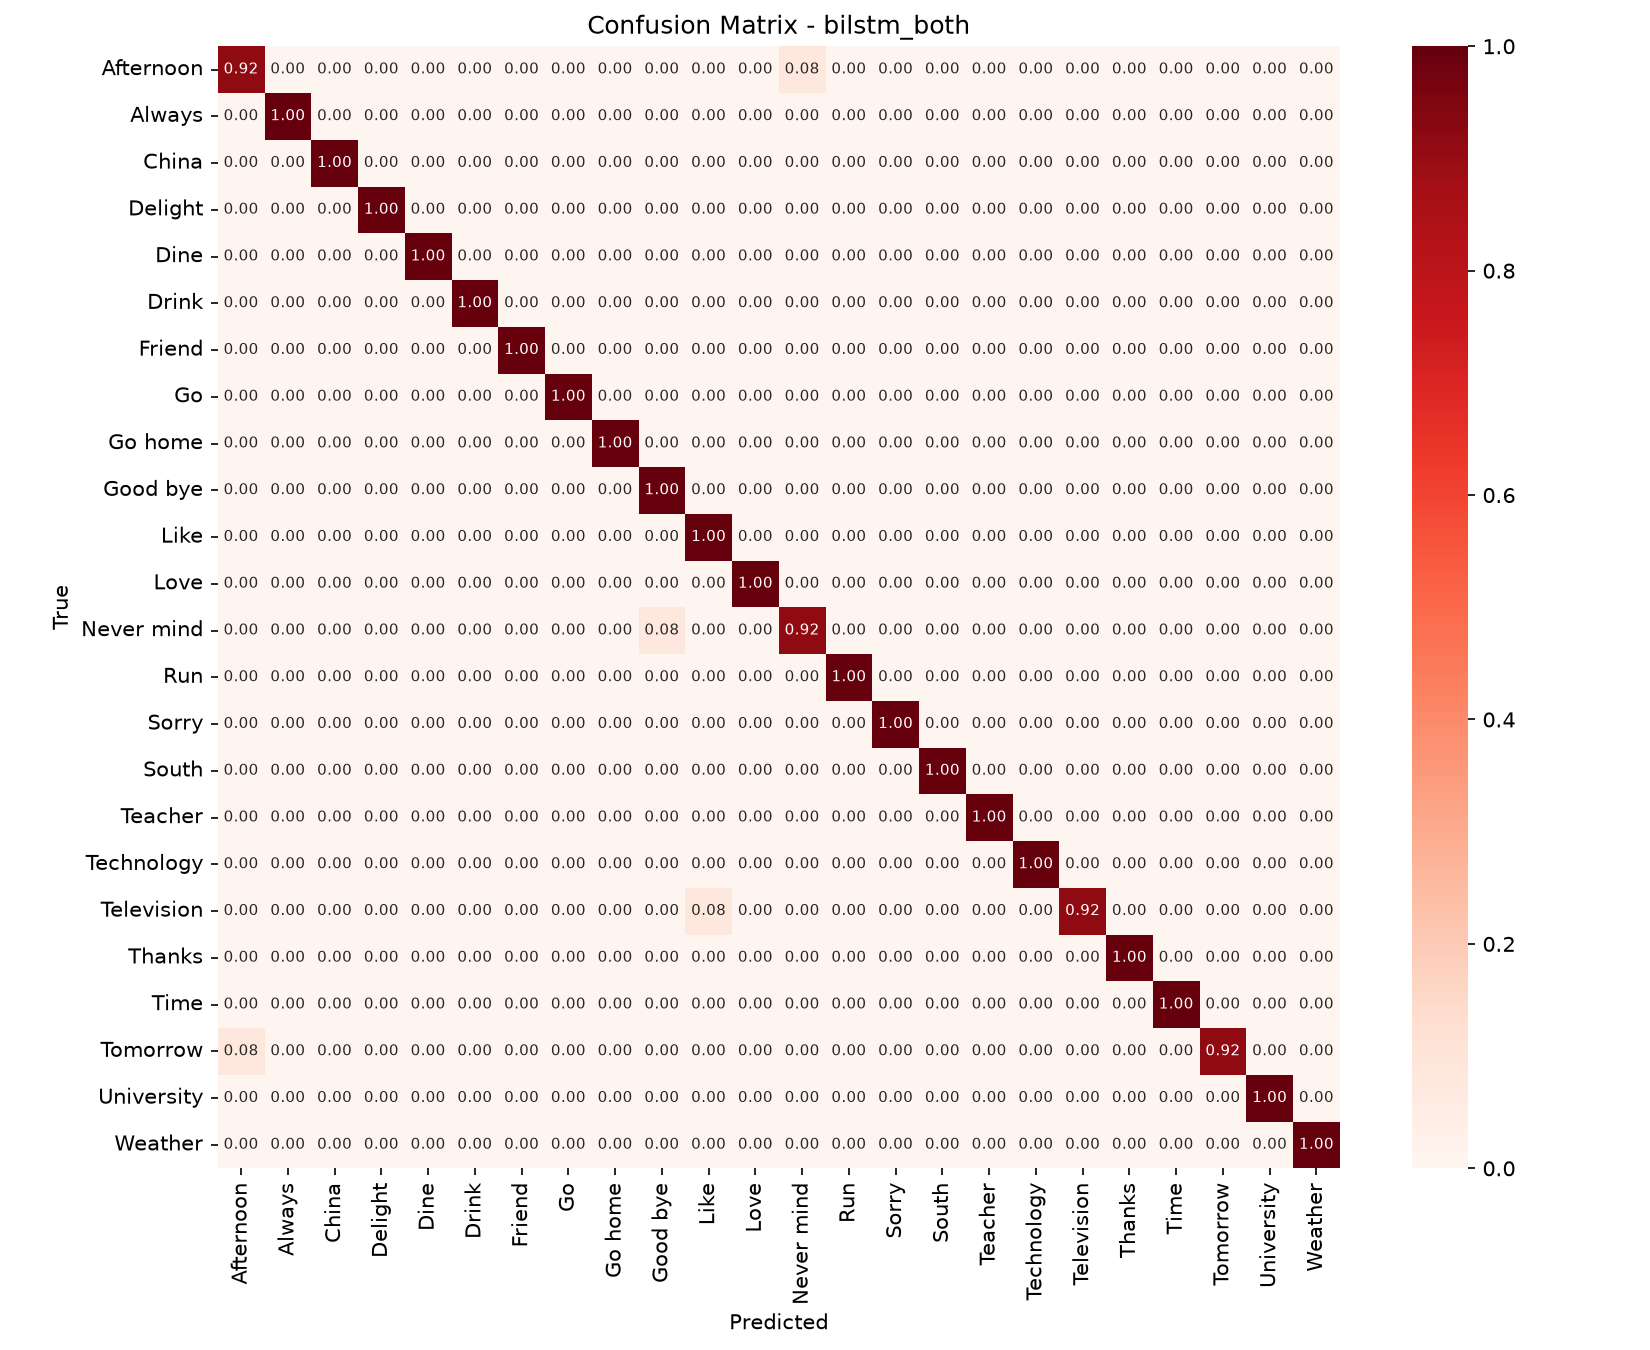
\includegraphics[width=0.85\textwidth]{bilstm_both_cm.png}
\caption{主模型的 24 类手语混淆矩阵（行归一化）}
\label{fig:cm}
\end{figure}

主模型在 288 个测试样本中仅错分 4 个，准确率 98.61\%。全部误分类样本见表~\ref{tab:errors}，各类别召回率见表~\ref{tab:perclass}。

\begin{table}[htbp]\centering
\caption{主模型的全部误分类样本}
\label{tab:errors}
\begin{tabular}{lcc}
\toprule
真实类别 & 预测类别 & 次数 \\
\midrule
Tomorrow & Afternoon & 1 \\
Television & Like & 1 \\
Never mind & Good bye & 1 \\
Afternoon & Never mind & 1 \\
\bottomrule
\end{tabular}
\end{table}

\begin{table}[htbp]\centering
\caption{各类别召回率（主模型 Bi-LSTM 融合，按召回率升序）}
\label{tab:perclass}
\begin{tabular}{lccc}
\toprule
手语类别 & 测试样本数 & 正确数 & 召回率(\%) \\
\midrule
Afternoon & 12 & 11 & 91.7 \\
Never mind & 12 & 11 & 91.7 \\
Tomorrow & 12 & 11 & 91.7 \\
Television & 12 & 11 & 91.7 \\
Dine & 12 & 12 & 100.0 \\
Drink & 12 & 12 & 100.0 \\
China & 12 & 12 & 100.0 \\
Always & 12 & 12 & 100.0 \\
Go & 12 & 12 & 100.0 \\
Go home & 12 & 12 & 100.0 \\
Like & 12 & 12 & 100.0 \\
Good bye & 12 & 12 & 100.0 \\
Love & 12 & 12 & 100.0 \\
Run & 12 & 12 & 100.0 \\
Friend & 12 & 12 & 100.0 \\
Delight & 12 & 12 & 100.0 \\
South & 12 & 12 & 100.0 \\
Sorry & 12 & 12 & 100.0 \\
Technology & 12 & 12 & 100.0 \\
Teacher & 12 & 12 & 100.0 \\
Thanks & 12 & 12 & 100.0 \\
Time & 12 & 12 & 100.0 \\
University & 12 & 12 & 100.0 \\
Weather & 12 & 12 & 100.0 \\
\bottomrule
\end{tabular}
\end{table}


%=====================================================================
\section{最优模型与数据文件}

\subsection{模型选型}

综合各实验，给出两类“最优”：

\begin{itemize}[leftmargin=2em]
\item \textbf{综合性能最优模型}：\textbf{TCN}（多模态融合），测试准确率 \textbf{99.65\%}，参数量仅 0.30\,M，收敛快（6 轮）。对应权重 \texttt{outputs/checkpoints/model\_tcn.pt}。
\item \textbf{论文复现主线模型}：\textbf{双分支 Bi-LSTM 融合}，源论文参数下测试准确率 98.61\%；经参数调节将 Batch Size 由 50 调整为 32 后可达 \textbf{99.31\%}（学习率 $10^{-3}$、Batch Size 32、Dropout 0.3）。对应权重 \texttt{outputs/checkpoints/sweep\_batch\_size=32.pt}。
\end{itemize}

\subsection{相关数据文件}

\begin{table}[htbp]\centering
\caption{最优模型及相关 CSV 数据文件}
\label{tab:files}
\begin{tabular}{ll}
\toprule
文件 & 内容 \\
\midrule
\texttt{checkpoints/model\_tcn.pt} & TCN 最优模型权重 \\
\texttt{checkpoints/bilstm\_both.pt} & Bi-LSTM 主模型权重 \\
\texttt{results/model\_compare.csv} & 模型对比汇总（准确率/精确率/F1/参数量） \\
\texttt{results/modality\_compare.csv} & 多模态对比汇总 \\
\texttt{results/ablation.csv} & 消融实验汇总 \\
\texttt{results/param\_sweep\_all.csv} & 参数调节实验汇总 \\
\texttt{results/*\_history.csv} & 各次训练逐轮 Loss / Accuracy 记录 \\
\texttt{results/*\_test\_pred.csv} & ~各次实验的测试集逐样本预测结果 \\
\bottomrule
\end{tabular}
\end{table}

%=====================================================================
\section{结果分析与讨论}
\label{sec:analysis}

\subsection{模型优势}

\begin{enumerate}[leftmargin=2em]
\item \textbf{双分支结构适配异构模态。} 手套信号（200\,Hz、400 点）与 sEMG（1000\,Hz、1950 点）采样率与时间长度均不同，双分支分别建模避免了强制对齐带来的信息损失。
\item \textbf{判别能力强且训练稳定。} 仅需约 29 轮即收敛，训练与验证曲线无过拟合迹象。
\item \textbf{轻量化替代方案可行。} TCN/CNN 以约 1/50 的参数量达到同等精度，为部署到可穿戴端侧设备提供了现实路径。
\end{enumerate}

\subsection{易混淆手语及原因}

本实验在主模型训练前，先对 24 个类别做了类间相似度分析（以每类 120 个样本的通道均值向量计算 Pearson 相关系数）。结果发现若干高度相似的类别对，其中最相似的是 \textbf{Teacher--Tomorrow（$r=0.958$）}、Tomorrow--Weather（$0.924$）、China--Tomorrow（$0.862$）、\textbf{Like--Television（$0.857$）}。

后续实测的误分类结果印证了这一预测：

\begin{itemize}[leftmargin=2em]
\item \textbf{Television $\rightarrow$ Like}：正是相似度分析中排序靠前的类别对（$r=0.857$），两者在手套通道上的均值特征高度相关；
\item \textbf{Tomorrow $\rightarrow$ Afternoon}、\textbf{Afternoon $\rightarrow$ Never mind}、\textbf{Never mind $\rightarrow$ Good bye}：均落在上述高相似簇内；
\item 召回率最低的 4 类（均为 0.917）——Afternoon、Never mind、Tomorrow、Television——恰好就是这些高相似簇的成员。
\end{itemize}

\textbf{原因分析}：这些手语在手指弯曲与手掌姿态的传感器响应上高度接近（例如需要相似的手型变化幅度），而在 2 秒窗口内的时序差异有限，导致特征空间中类间距离小。这属于手势本身运动学相似导致的固有困难，而非数据或模型缺陷。

\subsection{与源论文结果的对照与差异分析}
\label{sec:gap}

\begin{table}[htbp]\centering
\caption{与源论文（Advanced Science 2026, 13:e20586）的对照}
\label{tab:gap}
\small
\begin{tabular}{lccc}
\toprule
项目 & 源论文 & 本复现 & 判定 \\
\midrule
融合准确率 & 99.65\% & 98.61\%（Bi-LSTM）/ 99.65\%（TCN） & 复现成功 \\
仅应变/压力 & 83.75\% & 98.26\% & 显著分歧 \\
仅 sEMG & 88.02\% & 91.32\% & 接近 \\
参考架构 & 双分支 Bi-LSTM 融合 & 已复现 & 一致 \\
训练超参 & AdamW / 50 / $10^{-3}$ / 0.3 & 已复现 & 一致 \\
\bottomrule
\end{tabular}
\end{table}

\textbf{已排除的解释}：经独立核验，划分正确（三集合互斥且完备）、标签正确（近邻跨类数为 0）、归一化统计量无泄漏；近重复效应经量化为 $+0.52$\,pp，不足以解释 14\,pp 的差距。

\textbf{最可能的原因}：源论文的单模态对比实验（其 Fig.~S25）可能并非“单独训练一个单模态模型”，而是\textbf{在已训练的融合模型上做测试时模态剪枝}（将另一分支输入置零）。后者难度显著更高，因为模型已学会依赖两支输入。由于该论文的 Supporting Information 在本地不可得，此推测无法核实，故本报告不作定论。

\textbf{一个值得注意的旁证}：本实验在剔除近重复样本后，sEMG 单模态准确率为 \textbf{89.50\%}，与论文报告的 88.02\% 更为接近，提示差异可能部分来自评测条件的松紧程度。

\subsection{局限性与改进方向}

\begin{enumerate}[leftmargin=2em]
\item \textbf{统计效力有限}：测试集仅 288 样本，95\% 置信区间约 $\pm1$\,pp。第 8 节对模型间差异采用 4 个随机种子的统计（Bi-LSTM $98.96\pm0.40$\,\%）而非单次结果。
\item \textbf{近重复效应}：27.4\% 的测试样本在训练集中存在近似重复件，使整体准确率存在约 $+0.5$\,pp 的乐观偏差。改进：采用“近重复分组划分”，将相似样本归入同一集合。
\item \textbf{sEMG 信号质量}：约 65\% 的能量集中于 1--20\,Hz 漂移与 48.17\,Hz 工频干扰。\textbf{该推测已在第 11.2 节被实验推翻}：施加带通 + 陷波滤波后，sEMG 单模态准确率由 89.24\% 降至 75.69\%（$-13.55$\,pp），说明低频成分携带判别信息而非噪声。
\item \textbf{融合机制未生效}：第 9.2 节推理剪枝与第 11 节模态 Dropout 共同证明本模型的 sEMG 分支\textbf{在分类决策中完全未被使用}，所谓“多模态融合”实质等价于单模态。改进方向不在输入侧，而在训练机制。
\end{enumerate}

%=====================================================================
\section{结论}

本实验完成了 24 类中国手语识别任务的全流程实现与五组系统性实验（累计 31 组训练）：

\begin{enumerate}[leftmargin=2em]
\item 构建了完整的读取—预处理—划分—训练—评估流水线，划分严格满足 8:1:1 且以 \texttt{.pkl} 为单位，无数据泄漏；
\item 主模型（双分支 Bi-LSTM 融合）单次取得测试集准确率 \textbf{98.61\%}，各项指标一致；4 个随机种子的重复实验给出 \textbf{$98.96\pm0.40$\,\%}，TCN 对比模型为 \textbf{$99.42\pm0.40$\,\%}（单次最高 99.65\%），复现了源论文的融合精度水平；
\item 消融实验量化了分支内 FC（$-2.43$\,pp）、时序深度（$-3.82$\,pp）与拼接融合（$-1.04$\,pp）的贡献；
\item 参数调节实验表明：Batch Size 32 最优（99.31\%）；并验证了\textbf{单项最优叠加并不成立}——三项最优组合反而因过拟合降至 98.26\%，最终采用学习率 $10^{-3}$、Batch 32、Dropout 0.3；
\item \textbf{融合机制实验}：推理剪枝显示去掉 sEMG 后模型预测逐样本不变（288/288），模态 Dropout 亦无法改变该行为；滤波实验推翻了"低频是噪声"的直觉（sEMG 单模态 $-13.55$\,pp）；Oracle 上界分析表明五组配置中有四组的融合理论上限即等于当前成绩；
\item 定位了易混淆手语类别（Television/Like、Tomorrow/Afternoon/Never mind 等），并用类间相似度分析解释了成因。
\end{enumerate}

如实报告与源论文在单模态结果上的分歧、测试集规模带来的统计不确定性、数据中的近重复效应、
以及\textbf{融合机制本身未能生效}这一负面发现，是本报告在方法严谨性方面的自觉要求。

\vspace{4pt}
\noindent\textbf{最终结论}：本复现表明，源论文"多模态融合显著优于单模态（$+15.9$\,pp）"的核心论点在
本数据集上\textbf{不成立}——手套单模态已接近性能天花板（98\%$\sim$99\%），融合模型的 sEMG 分支从未被训练利用。
该结论由四组相互独立的证据支撑：推理剪枝（288/288 预测逐样本不变）、
模态 Dropout（训练准确率被钉在 0.7617，即优化器宁可牺牲 25\% 样本也不学 sEMG）、
Oracle 上界（5 组中 4 组净空间为 0.00\,pp）、以及多种子统计（模型间差异小于种子标准差 0.40\,pp）。
分歧的根源不在融合机制的实现，而在于\textbf{主导模态现象}——当一路模态已近乎解决全部可分样本时，
第二路模态不再有可贡献的空间。

\end{document}
